% mnras_template.tex
%
% LaTeX template for creating an MNRAS paper
%
% v3.0 released 14 May 2015
% (version numbers match those of mnras.cls)
%
% Copyright (C) Royal Astronomical Society 2015
% Authors:
% Keith T. Smith (Royal Astronomical Society)

% Change log
%
% v3.0 May 2015
%    Renamed to match the new package name
%    Version number matches mnras.cls
%    A few minor tweaks to wording
% v1.0 September 2013
%    Beta testing only - never publicly released
%    First version: a simple (ish) template for creating an MNRAS paper

%%%%%%%%%%%%%%%%%%%%%%%%%%%%%%%%%%%%%%%%%%%%%%%%%%
% Basic setup. Most papers should leave these options alone.
\documentclass[a4paper,fleqn,usenatbib]{mnras}

% MNRAS is set in Times font. If you don't have this installed (most LaTeX
% installations will be fine) or prefer the old Computer Modern fonts, comment
% out the following line
\usepackage{newtxtext,newtxmath}
% Depending on your LaTeX fonts installation, you might get better results with one of these:
%\usepackage{mathptmx}
%\usepackage{txfonts}

% Use vector fonts, so it zooms properly in on-screen viewing software
% Don't change these lines unless you know what you are doing
\usepackage[T1]{fontenc}
\usepackage{ae,aecompl}

\usepackage{mhchem}



\usepackage{graphicx}
\usepackage{subcaption}
\usepackage{float}
\usepackage{gensymb}
\usepackage{color}
\usepackage{booktabs,chemformula}
\usepackage[export]{adjustbox}

\usepackage{verbatim}
\usepackage{tabularx}

\usepackage{caption}
\usepackage{subcaption}
\usepackage{amsmath}

\usepackage{tikz}
\usepackage{hyperref}
\usepackage{longtable}
\usepackage{color}
\newcommand{\todo}[1]{\textcolor{red}{#1}}


\newcommand{\LamostGiants}{454,180}
\newcommand{\project}[1]{#1}
\newcommand{\lamost}{\project{LAMOST}}
\newcommand{\apogee}{\project{APOGEE}}

\newcommand{\tc}{\project{The Cannon}}

\newcommand{\teff}{T_{\rm eff}}
\newcommand{\logg}{\log_{10}(g/{\rm cm\,s}^{-2})}
\let\ACMmaketitle=\maketitle
\renewcommand{\maketitle}{\begingroup\let\footnote=\thanks \ACMmaketitle\endgroup}
%%%%%%%%%%%%%%%%%%% TITLE PAGE %%%%%%%%%%%%%%%%%%%

% Title of the paper, and the short title which is used in the headers.
% Keep the title short and informative.
\title[Mg--K stars in LAMOST]{On the discovery of K-enhanced and Mg-depleted stars throughout the Milky Way\footnote{This paper includes data gathered with the 6.5 meter Magellan Telescopes located at Las Campanas Observatory, Chile.}}

% The list of authors, and the short list which is used in the headers.
% If you need two or more lines of authors, add an extra line using \newauthor
\author[Kemp et al.]{Alex J. Kemp,$^{1}$\thanks{E-mail: ajkem1@student.monash.edu}
Andrew R. Casey,$^{1,2}$
Matthew T. Miles,$^{1}$
Brodie J. Norfolk,$^{1}$\newauthor
John C. Lattanzio,$^{1}$
Amanda I. Karakas,$^{1}$
Kevin C. Schlaufman,$^{3}$
Anna Y.~Q. Ho,$^{4}$\newauthor
Christopher A. Tout,$^{1,5}$
Melissa Ness,$^{6}$
Alexander P. Ji$^{7}$
\\
% List of institutions
$^{1}$School of Physics \& Astronomy, Monash University, Clayton 3800, Victoria, Australia\\
$^{2}$Faculty of Information Technology, Monash University, Clayton 3800, Victoria, Australia\\
$^{3}$Department of Physics and Astronomy, Johns Hopkins University, Baltimore, MD 21218, USA\\
$^{4}$Cahill Center for Astrophysics, California Institute of Technology, MC 249-17, 1200 E California Blvd, Pasadena, Ca, 91125, USA\\
$^{5}$Institute of Astronomy, Madingley Road, Cambridge, CB3 0HA, United Kingdom\\
$^{6}$Columbia University\\
$^{7}$Carnegie Observatories
}
% These dates will be filled out by the publisher
\date{Accepted 2018 XX XX. Received 2018 YY YY; in original form 2018 ZZ ZZ}

% Enter the current year, for the copyright statements etc.
\pubyear{2018}


\begin{document}
\label{firstpage}
\pagerange{\pageref{firstpage}--\pageref{lastpage}}
\maketitle

% Abstract of the paper
%The detailed chemical composition of a star acts as a fossil record of the conditions when it formed. 

\begin{abstract}
Stars with unusual elemental abundances offer clues about rare astrophysical events or nucleosynthetic pathways. Stars with significantly depleted magnesium and enhanced potassium ($[{\rm Mg}/{\rm Fe}] < -0.5$; $[{\rm K}/{\rm Fe}] > 1$) have to date only been found in the massive globular cluster NGC~2419 and, to a lesser extent, NGC~2808. The origin of this abundance signature remains unknown, as does the reason for its apparent exclusivity to these two globular clusters. Here we present
112 field stars, identified from \LamostGiants\ \lamost\ giant stars using a data-driven model (\tc), that show significantly enhanced [K/Fe] and likely depleted [Mg/Fe] abundance ratios.
Our sample spans a range of metallicities ($-1.5 < [{\rm Fe}/{\rm H}] < 0.3$) yet none show abundance ratios of [K/Fe] or [Mg/Fe] that are as extreme as those observed in NGC~2419. 
We conclude that the nucleosynthetic process producing the anomalous abundances in [K/Fe] and [Mg/Fe] probably occurs at a wide range of metallicities. This would suggest that pollution scenarios that are limited to early epochs (such as Population III supernovae) are an unlikely explanation, although they cannot be ruled out entirely. This sample is expected to help guide modelling  attempts to explain the origin of the Mg--K abundance signature, which we show exists throughout the Milky Way.
\end{abstract}

% Select between one and six entries from the list of approved keywords.
% Don't make up new ones.
\begin{keywords}
methods: data analysis -- catalogues -- stars: chemically peculiar -- Galaxy: abundances -- Galaxy: evolution -- galaxies: globular clusters: individual: evolution
\end{keywords}

%%%%%%%%%%%%%%%%%%%%%%%%%%%%%%%%%%%%%%%%%%%%%%%%%%

%%%%%%%%%%%%%%%%% BODY OF PAPER %%%%%%%%%%%%%%%%%%

\section{Introduction}
\label{sec:intro}
NGC 2419 is the Milky Way's third most massive globular cluster, and its chemical composition makes it perhaps the most unusual star cluster in the Galaxy. Recent spectroscopic studies of red giant branch (RGB) stars in NGC 2419 revealed a strong anti-correlation between Mg and K abundances in nearly half of the studied stars, and weaker abundance relations in Si, Sc, Ca, Ti and V with Mg \citep{mucciarelli2012,cohenkirby2012}.

A targeted search looking for [K/Fe] in RGB and main sequence turn-off stars in other clusters (NGC 6752, NGC 6121, NGC 1904, NGC 104, NGC 6397, NGC 7099, and $\omega$ Centauri) and field stars concluded that all K abundance ratios fell within the bounds of the Mg-normal population in NGC 2419 \citep{carretta2013}, and no correlations between Mg and K were observed. Recent work by \cite{cerniauskas201747tuc} searched for unusual abundance patterns in Mg and K in NGC 104 through deriving abundances using 2df/HERMES spectra, and a more comprehensive study involving over 400 stars in NGC 104, NGC 6752, and NGC 6809 by \cite{mucciarelli2017K} using FLAMES spectra \citep{cerniauskas201747tuc} both found no correlations between Mg and K, and no significant intrinsic spreads in either Mg or K.

NGC 2808 is the only cluster, other than NGC 2419, where an anticorrelation between Mg and K has been observed. All four of NGC 2808's known Mg-depleted stars show an anti-correlation with K \citep{mucciarelli2015}, although the amplitude of these abundance ratios is far weaker than those found in NGC 2419. The fact that the Mg-K anti-correlation is apparently confined to these two globular clusters implies either a small population of unusual polluter stars, or a single extremely massive polluter star. If it were the cumulative effect of many pollution events that was responsible for the signal, it would be expected that the anomalous abundances would be common among globular clusters.

%Recently \cite{youngwooklee} used a Ca filter to identify two population in NGC 2419 corresponding to two generations of stars: G1, first generation metal poor stars, and G2, second generation stars displaying enhanced Ca and significantly increased He abundance ($\Delta Y = 0.19$). The Mg-depleted population identified previously was found to be contained with the G2 population.




%It has been suggested that NGC 2419's position and size, being both very massive and very distant from the Milky Way compared to many other globular clusters, aids it in retaining enriched material from explosive events \citep{mucciarelli2012}. It is also perhaps noteworthy that NGC 2808 is also one of the more massive globular clusters of the Milky Way, although it is far closer to the Galactic Centre. But if this unknown pollution event is common among globular clusters and the cause of its apparent exclusivity to NGC 2808 and NGC 2419 is enhanced ejecta retention due to high mass, then other massive clusters such as $\omega$ Centauri would also be expected contain the signature, which to date has not been observed.

%While it is plausible that the increased mass and greater distance from the gaseous disk of the Milky Way would cause a clusters first generation polluter stars to have an increased effect on the second generation of stars, this effect would apply to all ejecta (assuming comparable energies). So while it might be expected that second generation stars in clusters similar to NGC 2419 made up of more material processed by the first generation than other lighter globular clusters, it doesn't explain why the ejecta from the first generation was apparently dominated by this as yet unknown polluter object resulting in the Mg--K anti-correlation. In the opinion of the author, it is the identity and physical characterisation of this unknown polluter that is of the greatest scientific interest, with such a result also hopefully answering the question of the signatures uniqueness.

Beyond the intrinsic scientific value of identifying the mechanism responsible for the puzzling Mg--K anti-correlation, a satisfactory explanation for the Mg--K signature may also offer insight into the underestimation of K abundances in the Milky Way predicted by Galactic chemical evolution models \citep{kobayashi2011} or more broadly help to understand globular cluster formation and evolution. 

Here we use low resolution \lamost\ data to conduct the largest search to date for stars enhanced in potassium and depleted in magnesium. The discovery (or non-discovery) of such stars guides models that attempt to explain the Mg--K anti-correlation and related abundance phenomena. In particular, such a search provides strong evidence either for or against the uniqueness of the progenitor stars to globular clusters. In Section \ref{sec:method} we outline our methods to identify candidates enhanced in K and depleted in Mg, and the follow-up observations and abundance analysis for some of those candidates. In Section \ref{sec:discussion} we discuss our results and their implications for possible pollution mechanisms. 


%This study, which queries \LamostGiants\ \lamost\ giants for depleted Mg and enhanced K, seeks to provide additional information which can be used to guide and test models attempting to explain the Mg--K anti-correlation and related phenomena. The large sample size provides greater insight into the supposed exclusivity of the signature, and the stars identified present an important opportunity for follow up observations.


\section{Method \& Observations}
\label{sec:method}
\subsection{Candidate selection from \lamost\ spectra}
We used a set of \LamostGiants\ giant stars from the second \lamost\ data release \citep{luo2016vizier}. The spectra were placed at rest-frame on a common wavelength sampling from 3905\,\AA\ to 9000\,\AA\ and normalised by \citet{ho2017}. \tc\ \citep{ness2016,ho2017} was used to estimate effective temperature $\teff$, surface gravity $\logg$, metallicity [Fe/H], and mean $\alpha$-element abundance relative to iron [$\alpha$/Fe] using 9,952 stars in common between \lamost\ and the \apogee\ \citep{alam2015} survey. Unless otherwise stated, these transferred labels are those referred to throughout this study. For details regarding the preparatory work, model generation, and label transfer between the \apogee\ and \lamost\ surveys we direct the reader to \citet{ho2017}. 

We identified potential Mg-depleted and K-enhanced stars by searching for significant deviations in flux residuals. The flux residuals were calculated as the diference between the normalised \lamost\ flux and the best-fitting data-driven model flux from \tc\ ( $f_{\textrm{residual}} = f_{\textrm{data}} - f_{\textrm{model}}$). A positive residual implies a higher observed normalised flux than expected by the model (less stellar absorption than predicted by the model), while a negative residual implies a lower observed normalised flux than expected (more stellar absorption than predicted by the model). Figure \ref{posterchild} shows the \lamost\ spectrum and best-fitting model from \tc\ for candidate J034458.82+592955.1.

We fit a Gaussian profile to the flux residuals for all three absorption lines in the Mg triplet (5167\,\AA, 5172\,\AA, 5184\,\AA) as well as the K doublet (7665\,\AA, 7699\,\AA) for all \LamostGiants\ giants. For each star we recorded the profile amplitudes, wavelengths, widths, as well as associated measurement uncertainties of these quantities. We identified candidates by requiring that they match at least one of the following three quality filters:
\begin{enumerate}
\item We required the amplitude $A$ of the profile at the Mg 5184 \AA \ line to satisfy $A_{{\rm Mg} @ 5184} > 0.05$ and the amplitude of the profile at the K 7665\,\AA\ line to satisfy $A_{{\rm K}\,@\,7665} < -0.05$. Both amplitudes must also be measured at more than $3\sigma$ ($|A|/\sigma_{A} \geq 3$).
\item We required any two of the three Mg triplet lines to satisfy $A > 0.05$ and at least one K line to have $A < -0.05$, and for those amplitudes to have $|A|/\sigma_{A} \geq 3$.
\item We required any two of the three Mg triplet lines to have $A > 0$ and both K lines to have $A < 0$, and for the spectra to have a signal-to-noise ($S/N$) ratio of $S/N > 30$ in \lamost\ and a reported $\chi_{r}^2 < 3$ from \tc.
\end{enumerate} 
 
These filters identified 384 unique stars. We visually inspected every candidate (multiple times) and excluded stars that showed any evidence of being a false positive, including candidates that exhibited data reduction issues, apparent absorption that was narrower than the expected spectral resolution, as well as 75 stars that exhibited chromospheric emission at H$\alpha$, indicative of chromospheric activity which can cause deceptively strong spectral lines. The distilled catalogue contains 112 candidate stars with spectra consistent with enhancements in K and depletions in Mg.

We note that although telluric absorption would usually swamp the K doublet lines, the contributions of telluric features have been removed from \lamost\ spectra as part of the data reduction process conducted by \lamost\ \citep{luo2016vizier}. Subsequent examination of the radial velocities for the (manually vetted) sample showed no behaviour indicating that the [K/Fe] over-abundances identified were due telluric absorption.

We estimated [K/Fe] abundance ratios for all candidates by synthesising spectra to account for the flux residuals \citep{marcs,sme,vald,ispec}. We assume that absorption due to metals is accounted for by \tc, and deviations in flux around the potassium doublet are due to an increased [K/Fe] with respect to the model. We include a conservative 0.2\,dex systematic error floor  applied in quadrature with the fitting errors to account for some component of the flux differences not being from the abundance of K, but instead due to noise in the \lamost\ spectra. We applied the same method to estimate [Na/Fe] from \lamost\ spectra. We note that while enhancements in [K/Fe] or [Na/Fe] can be estimated by synthesising the flux residuals, we cannot easily estimate [Mg/Fe] depletions in the same manner because it is difficult to separate the flux contribution of [Mg/Fe] from [$\alpha$/Fe] in the data-driven model. For this reason, we will adopt [$\alpha$/Fe] as a conservative upper limit for [Mg/Fe].

%\todo{The presence of Na enhancements were visually estimated from the sample of 112 candidate stars' flux spectra. Flux-based estimates placed at most 40 of the 112 stars (35\%) as being likely Na enhanced targets.} Na abundances calculated from the \lamost\ spectra later revealed 30\% of the target stars with [Na/Fe] above 0.5\,dex. \todo{@andy add anything specific to Na abundance methods from LAMOST}.


\subsection{Follow-up observations with Magellan/MIKE}
High resolution spectra of three of the candidate stars selected based on observability (J075043.12+204658.0, J120032.60+024438.2 and J091825.49+172114.5) were obtained using Magellan/MIKE (Magellan Inamori Kyocera Echelle) \citep{shectman2003magellan,bernstein2003mike}. Exposure times were calculated to achieve S/N per pixel of 30 per pixel at 450\,nm, sufficient to verify the K-enriched and Mg-poor nature of these stars. We reduced the data using the \texttt{CarPy} package \citep{kelson2003}. Spline functions were used to continuum-normalize individual echelle orders, before combining them to produce a continuum-normalized spectrum that is contiguous from 350\,nm to 950\,nm. With the stellar parameters from \lamost, we calculated [K/Fe] and [Mg/Fe] abundances from individual atomic lines by measuring Gaussian profiles \citep{castelli2004,sneden,casey2014}. K lines were unaffected by telluric contamination in these candidates. The estimated abundances from Magellan/MIKE spectra are consistent (within the uncertainties) of our initial abundance determinations from \lamost\ (Figure \ref{KvsMg}).



\begin{figure*}
\centering
\begin{subfigure}{1\textwidth}
\centering
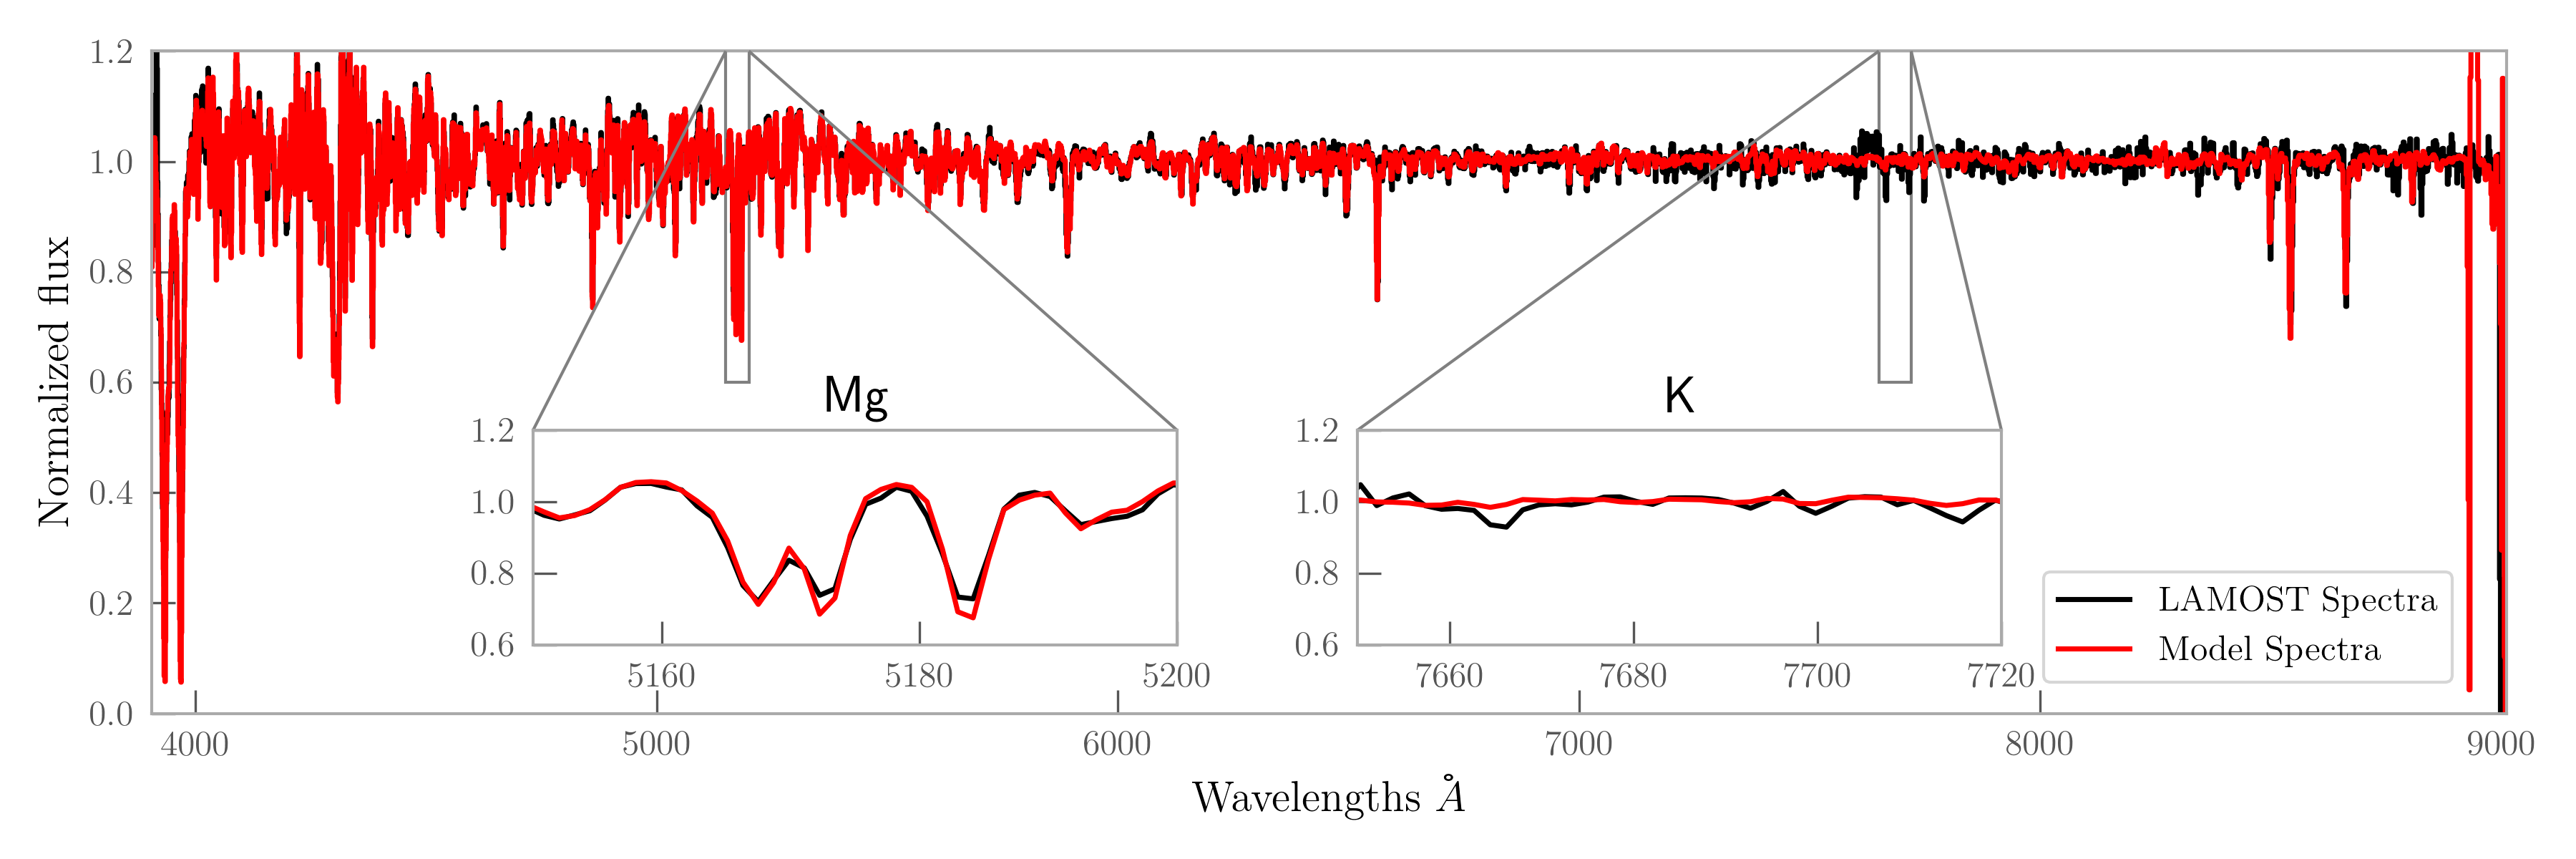
\includegraphics[width=\textwidth=1]{posterchild.png}
\caption{Mg-depleted, K-enhanced candidate J034458.82+592955.1.}
\end{subfigure}

\begin{subfigure}{1\textwidth}
\centering
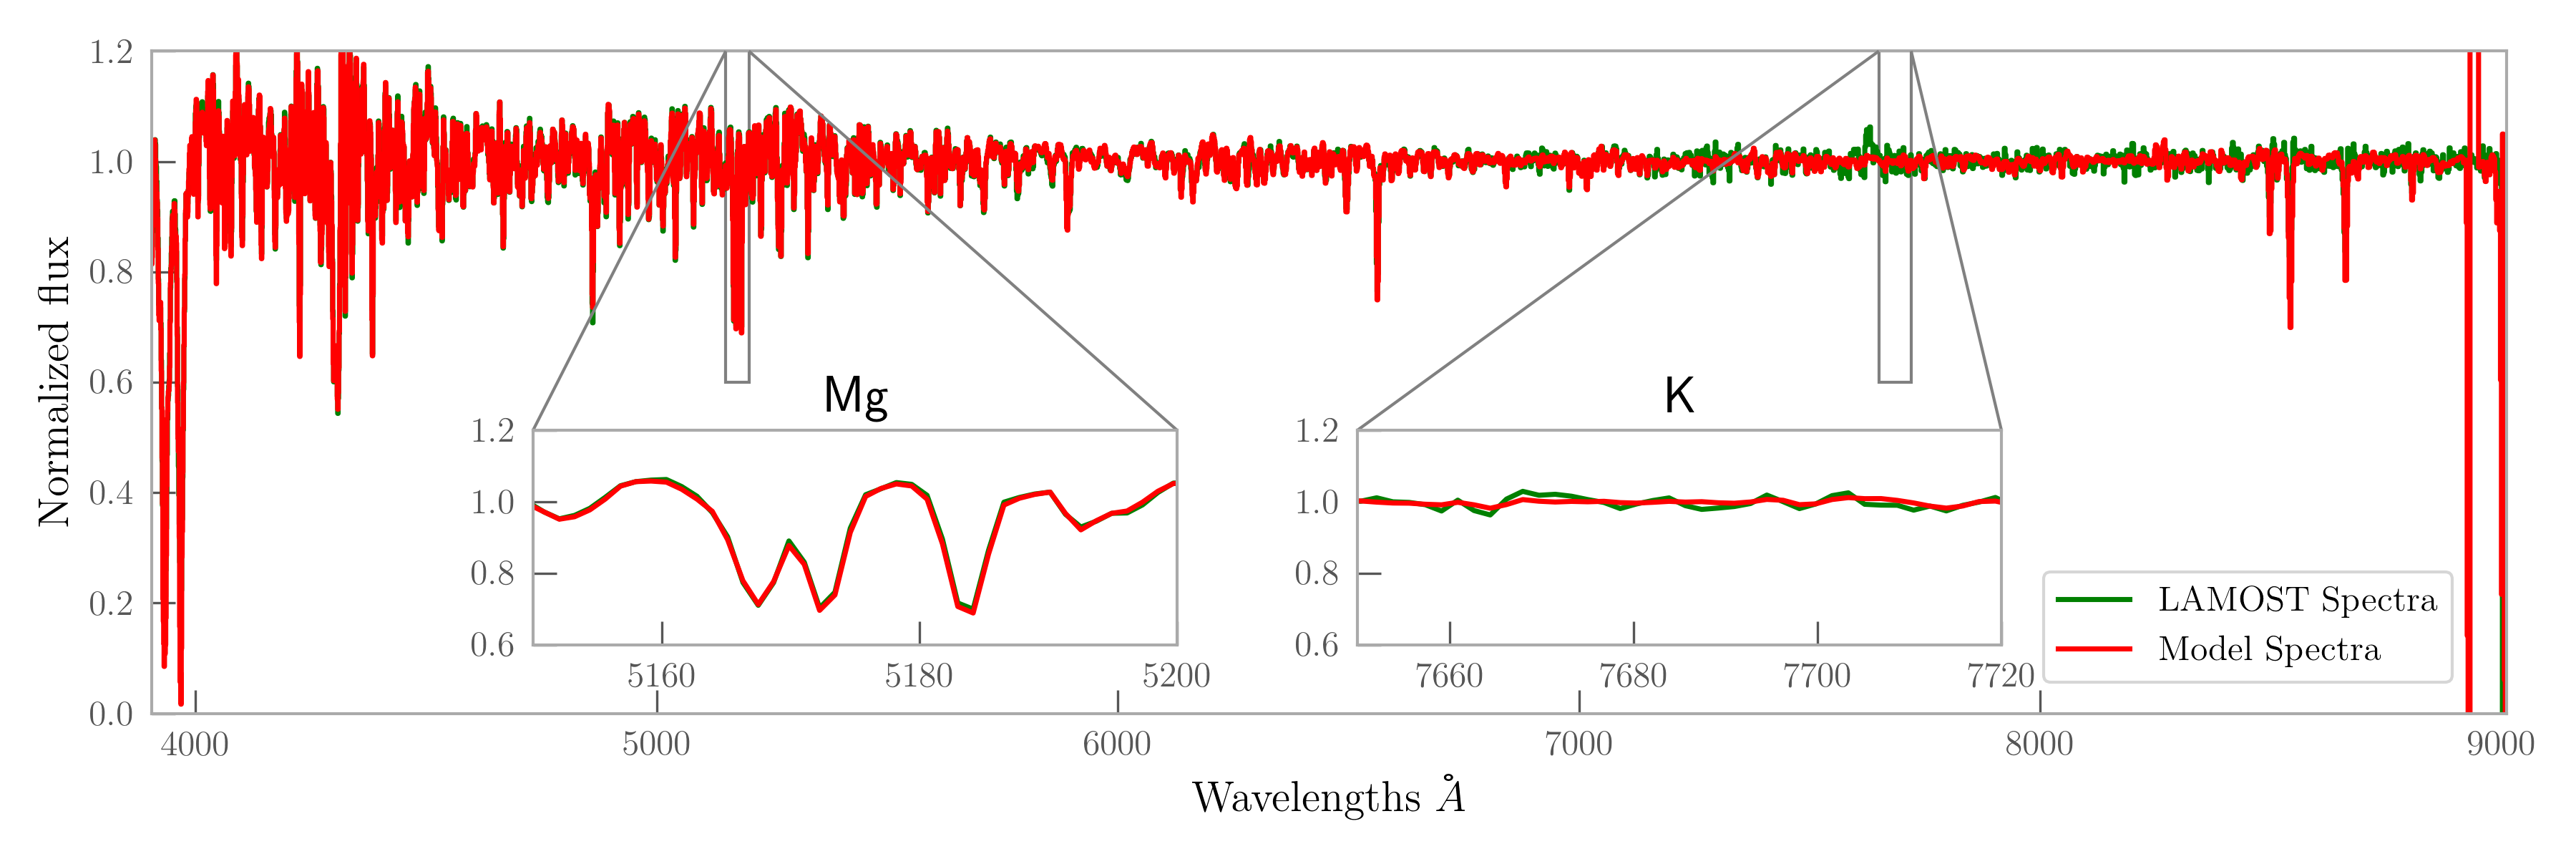
\includegraphics[width=\textwidth=1]{postermimic.png}
\caption{Mg-normal, K-normal star J163532.2+238131.54. }
\end{subfigure}

\caption{Normalised \lamost\ spectrum for the Mg-depleted and K-enhanced candidate J034458.82+592955.1 and for the comparable star J163532.2+238131.54. J163532.2+238131.54 was selected by minimising the similarity norm defined as $n=(\frac{\Delta \text{T}_{\text{eff}}}{1000})^2 +\Delta \text{logg} ^2 + \Delta \text{[Fe/H]}^2$. The data are shown in black and the best-fitting data-driven model from \tc\ is in red. We zoom in around the magnesium triplet and potassium doublet, which we used to identify Mg--K candidates. Note that $[\alpha/{\rm Fe}]$ is a label in \tc\ model used and J034458.82+592955.1 shows Mg depletions relative to the estimated [$\alpha$/Fe] value.}
\label{meshindepvisc}
\end{figure*}



\begin{figure}
	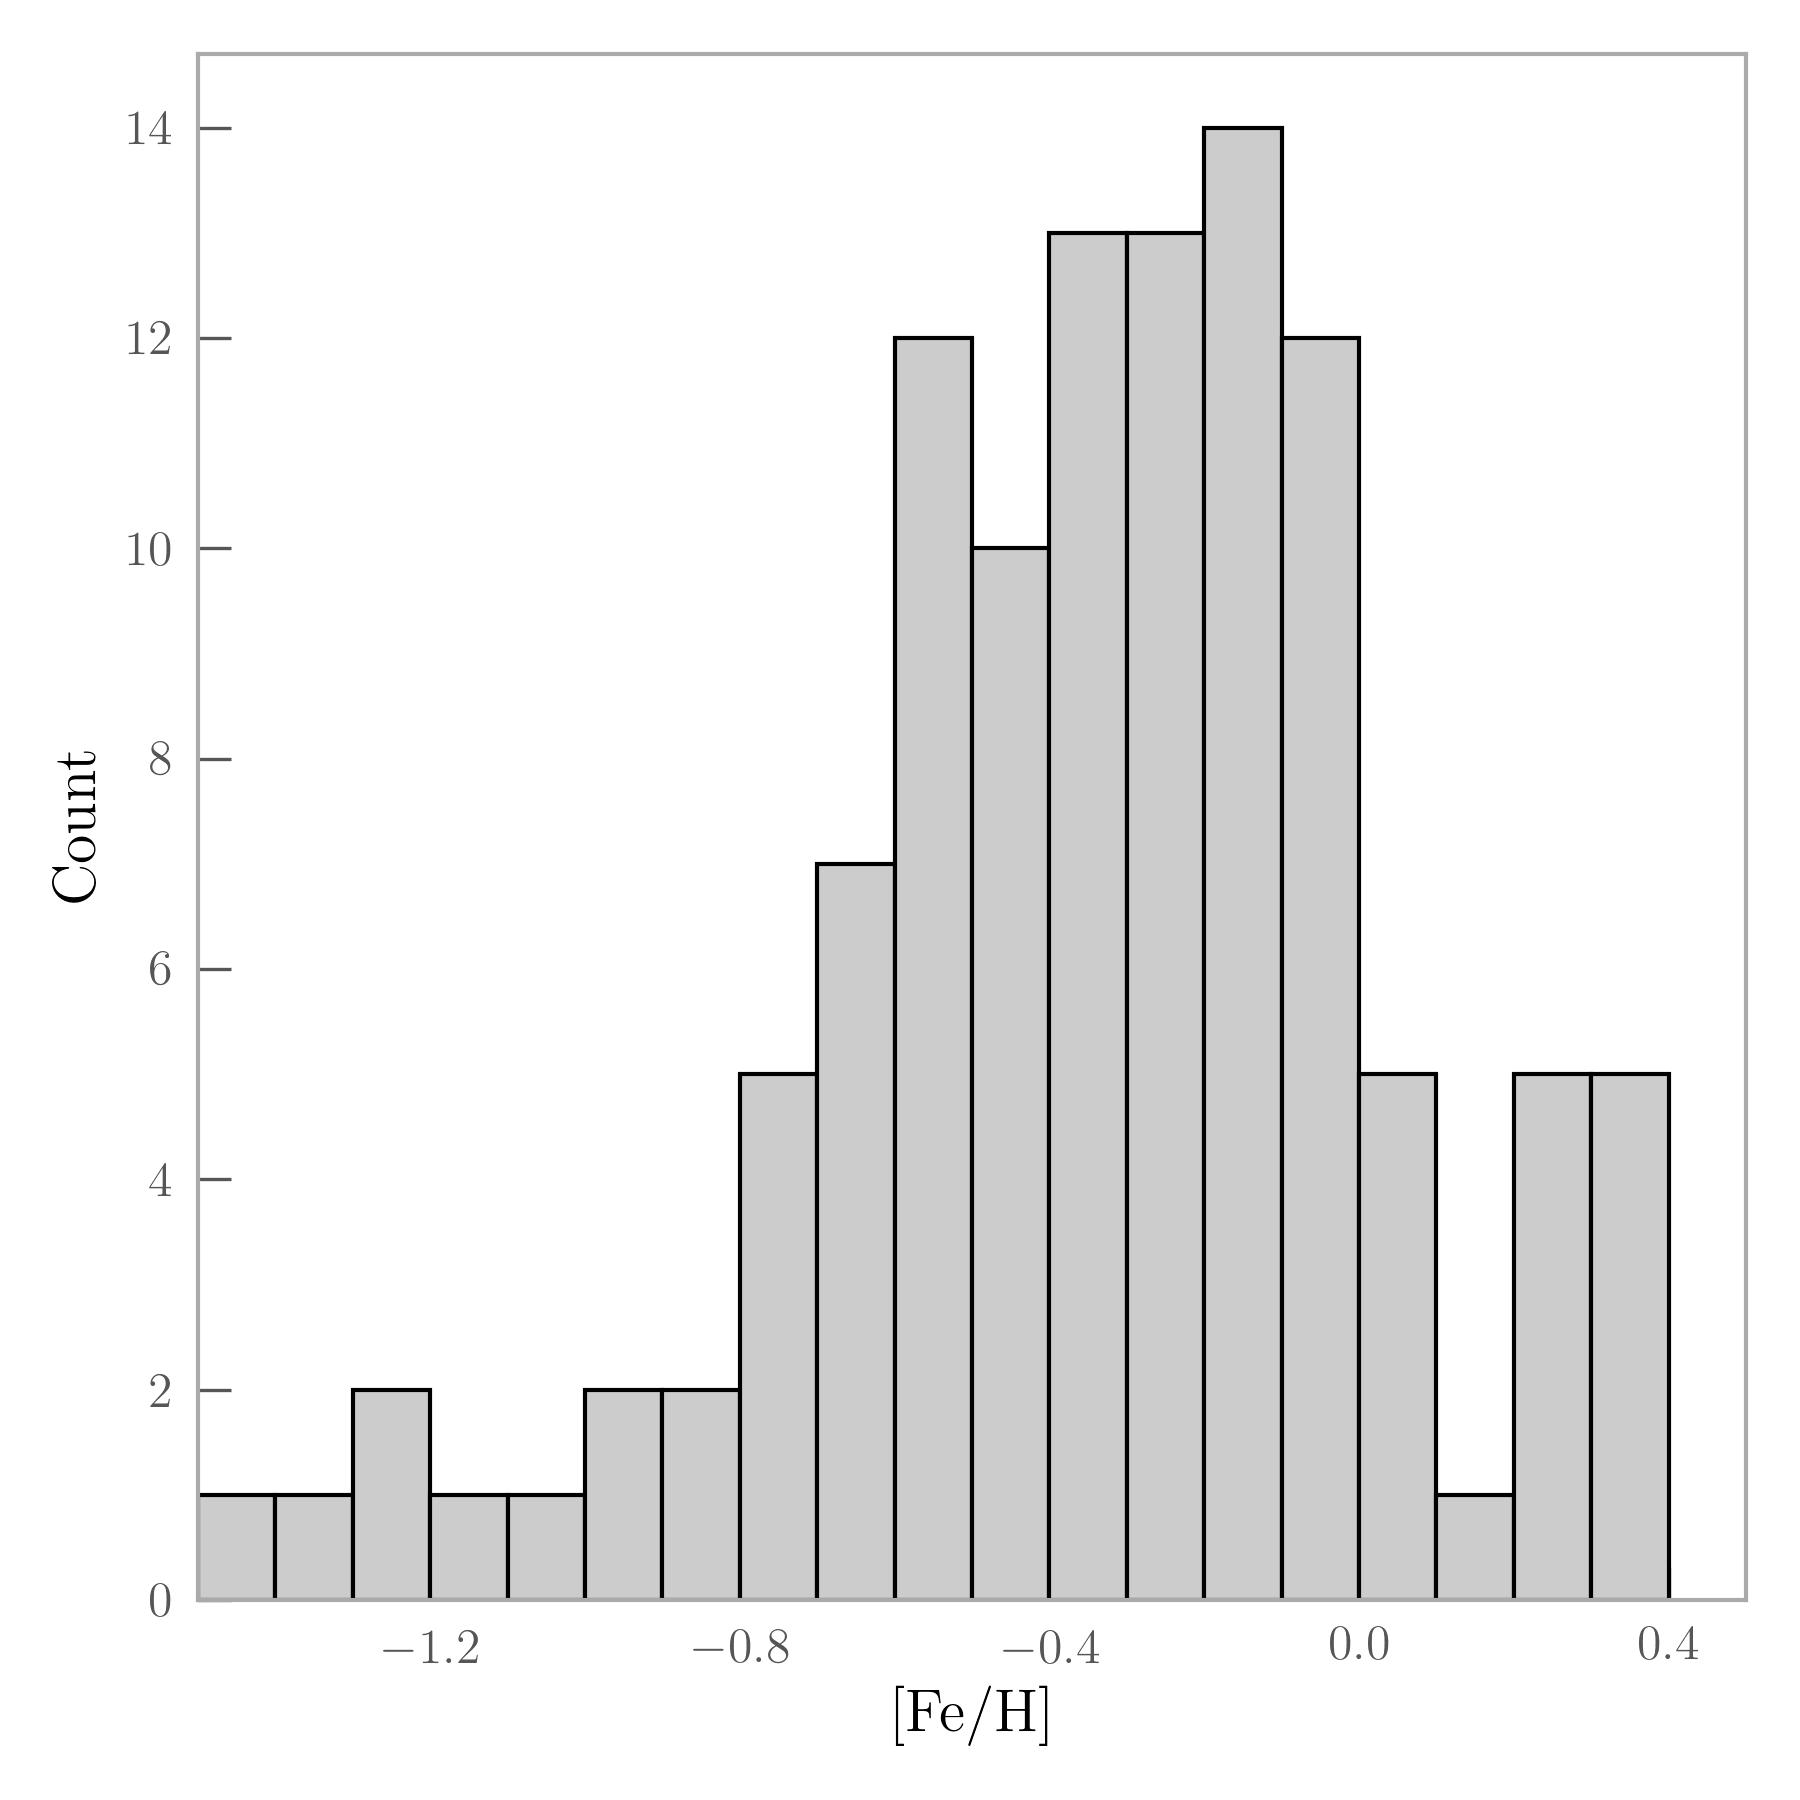
\includegraphics[width=\columnwidth]{mhist.png}
    \caption{Metallicity distribution for all 112 candidate stars identified with K-enhancement and Mg-depletion.}
    \label{mhist}
\end{figure}

\begin{figure}
	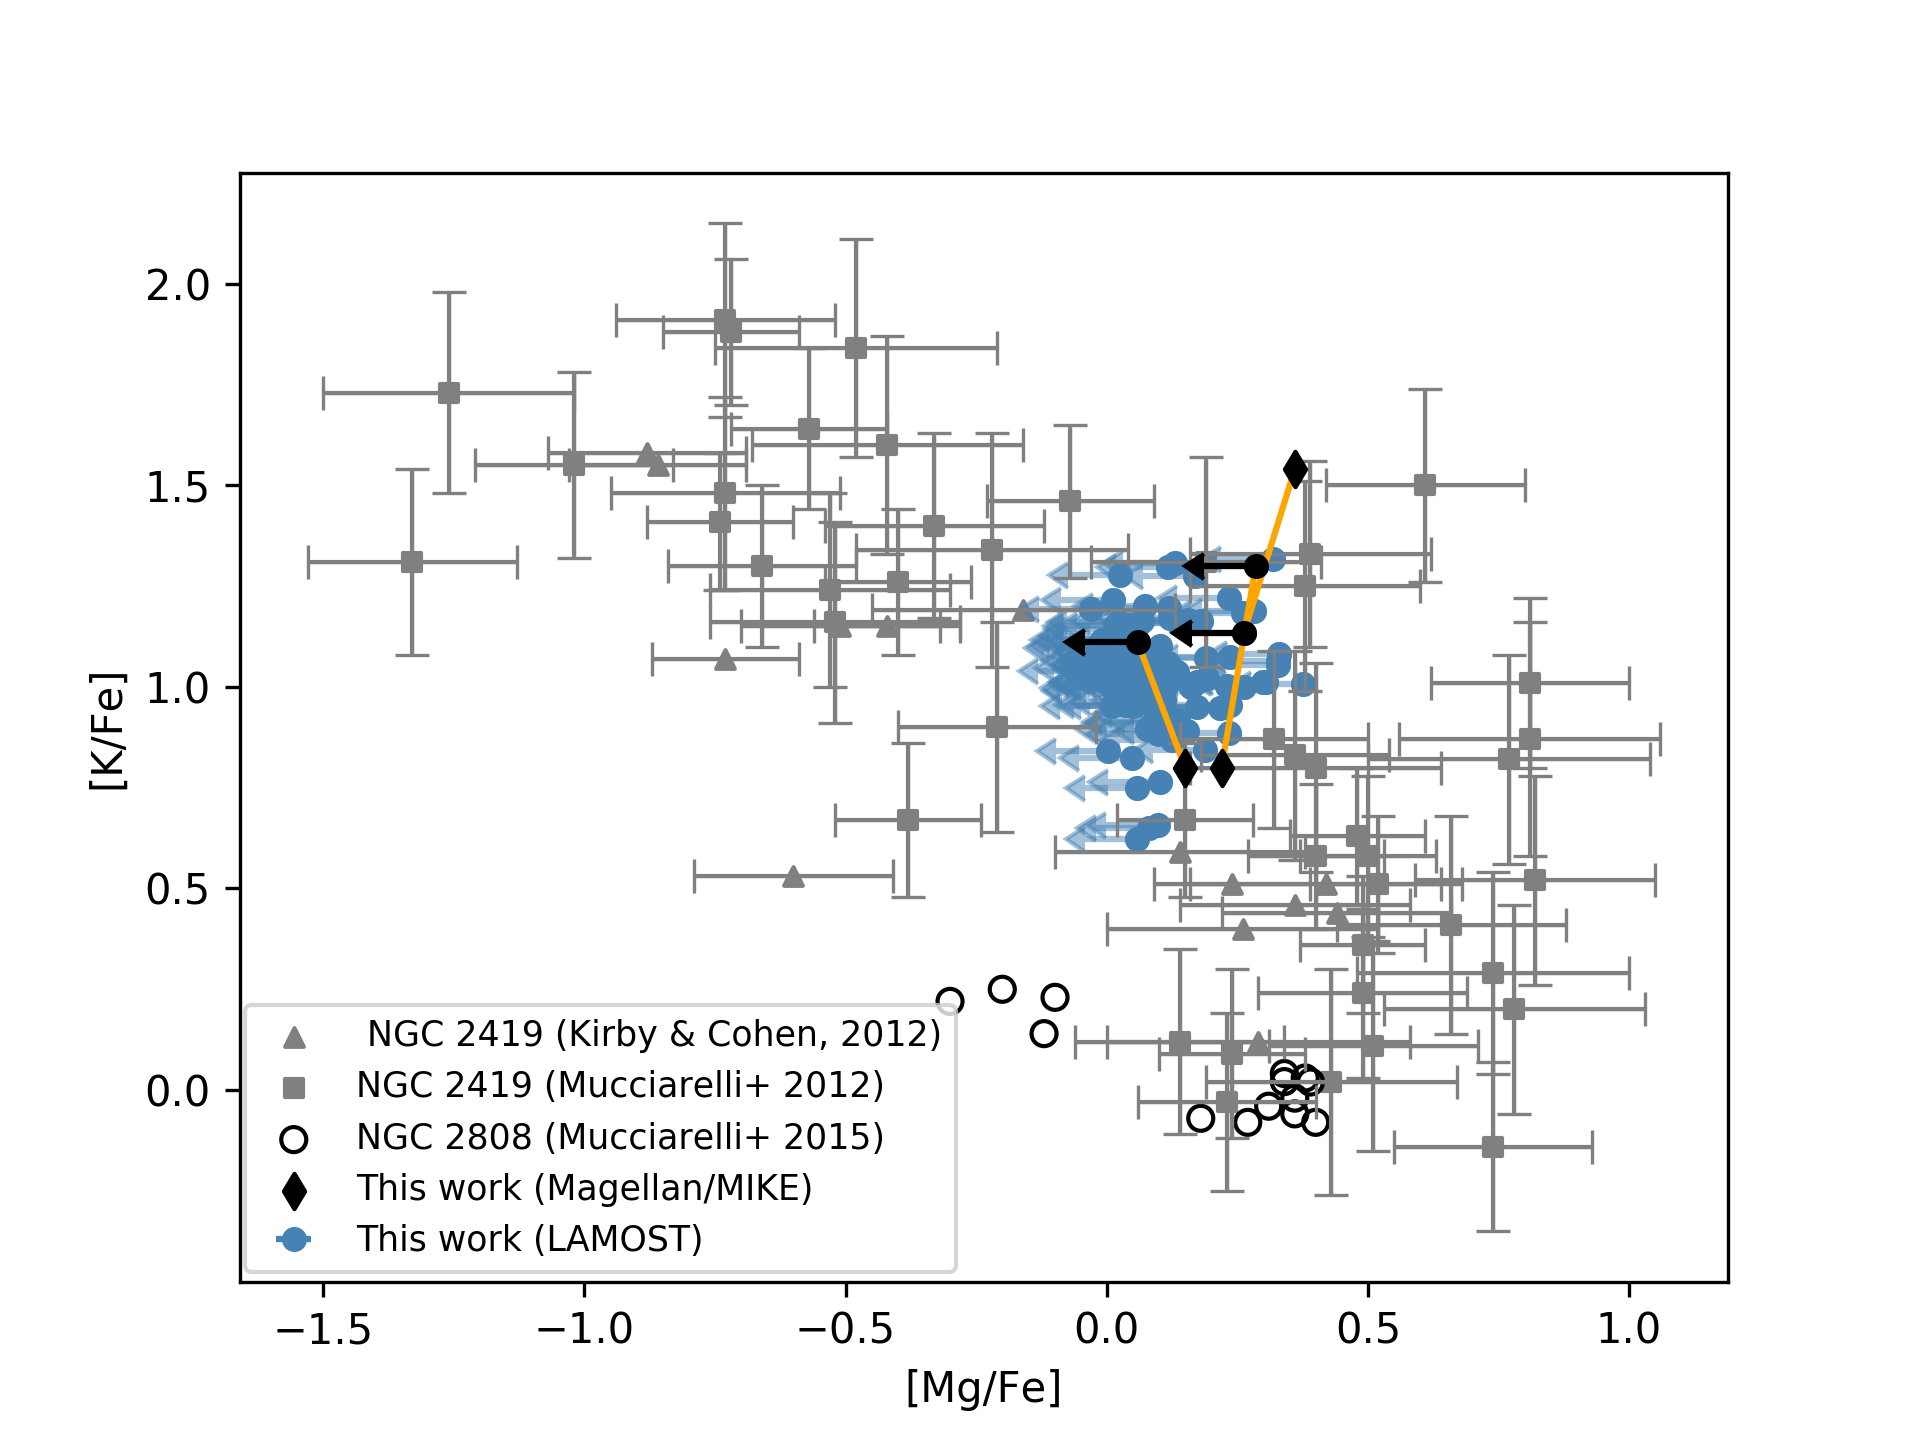
\includegraphics[width=\columnwidth]{KvsMg.png}
    \caption{[K/Fe] vs [$\alpha$/Fe] for the candidate stars, overlaid with [K/Fe] vs [Mg/Fe] abundances for NGC 2419 and NGC 2808 \citep{cohenkirby2012, mucciarelli2012, mucciarelli2015}. See Section \ref{sec:method} for discussion on the use of [$\alpha$/Fe] as a proxy for [Mg/Fe].} 
    \label{KvsMg}
\end{figure}

\begin{figure}
	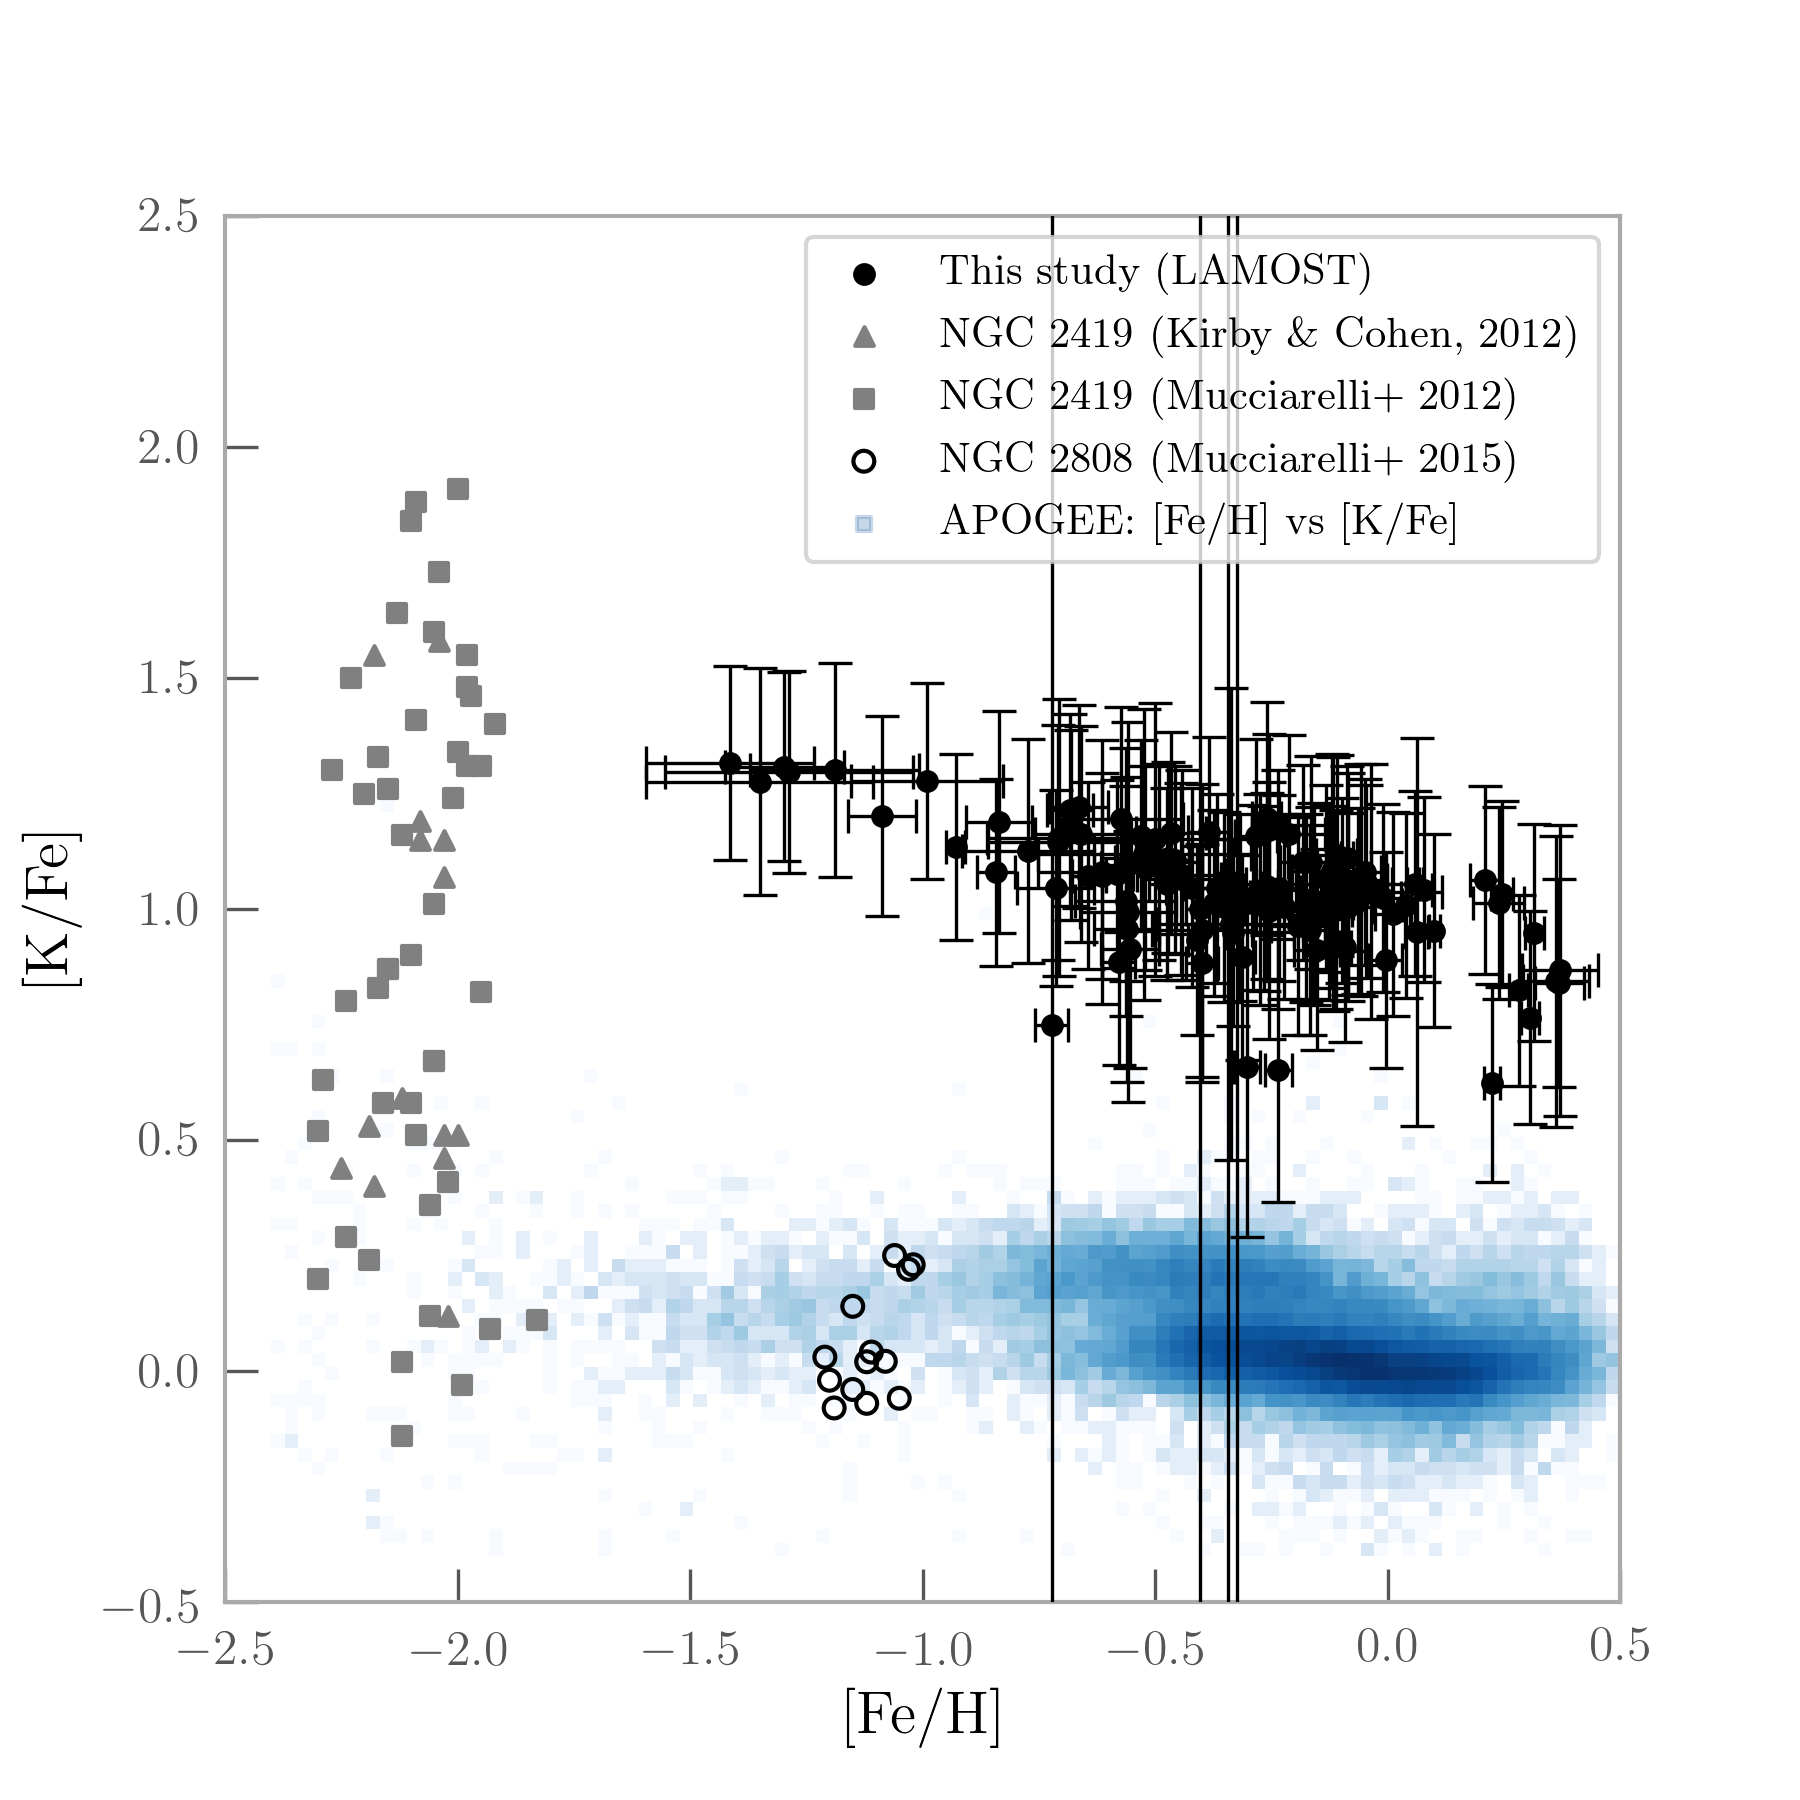
\includegraphics[width=\columnwidth]{KvsFe.png}
    \caption{[K/Fe] vs [Fe/H] for the candidate stars, overlaid with [K/Fe] vs [Fe/H] for NGC 2419 and NGC 2808 \citep{cohenkirby2012, mucciarelli2012, mucciarelli2015}. Metalicities for NGC 2808 are taken as the average metalicity for the cluster from \citet{harris1996}, as individual metallicities for these stars were not available.}
    \label{KvsFe}
\end{figure}

\section{Discussion}
\label{sec:discussion}

\subsection{Selection effects}
\label{sec:selectioneffects}

Our sample of \lamost\ giants carries with it certain selection effects from both the \apogee\ DR12 and \lamost\ samples. For example, metal-poor stars with [Fe/H] $\lesssim-2$ are mostly absent from our sample because they were too dissimilar from the training stars for label transfer from \apogee. Similarly, the target selection process for \lamost\ is not easily invertible so we do not consider selection effects present in \lamost\ beyond comparing the candidate stars' metallicity distribution with that of \cite{ho2017}. We find that the frequency of Mg--K stars is consistent (within the errors) of being flat with metallicity. We also note that our candidate stars are distributed across the entire giant branch, implying that the abundance signature is not associated with any single stage in evolution and that the chemical pattern we observe is not due to a violation of the assumption of local thermodynamic equilibrium.

\subsection{Association with known globular clusters}
\label{sec:globclustasoc}
We cross-matched our candidates with the positions of all known globular clusters \citep{harris1996}. The spread in metallicity (Figure \ref{mhist}) is consistent with all candidates being field stars. The distribution reflects the original \LamostGiants\ sample of giants from which the candidates were selected.
No candidates have [Fe/H] $\approx -2$, the approximate metallicity of NGC 2419, nor are there many stars with [Fe/H] $\approx -1$, the metallicity of NGC 2808. Thus, we conclude that the candidates are not restricted to any specific metallicity, particularly not just to the metallicities of NGC 2419 and NGC 2808.


\subsection{Detailed chemical abundances}
\label{sec:abundances}

Upon examining [Na/Fe] as estimated from the \lamost\ spectra, using the doublet around 5850 \AA, two distinct populations were observed: one population making up approximately 30 percent of the sample with [Na/Fe] > 0.5, significantly higher than typical Galactic abundances of [Na/Fe] $\lesssim$ 0.3 \citep{kobayashi2011}, and a second with [Na/Fe] consistent with typical Galactic abundances. However, the high [Na/Fe] abundance ratios we observe are possibly due to the effect of interstellar
dust contributing, as nearly every star with apparently enriched [Na/Fe] showed notably higher E(B-V) \citep{schlafly2011}, suggesting that the stellar absorption lines are blended with interstellar dust absorption. However, further investigation revealed no evidence of a diffuse interstellar band (DIB) impacting spectra around the Na doublet, nor Mg or K. It is worth mentioning briefly that the modelling work of \cite{prantzos2017} predicted an anti-correlation between Na and K in a 180\,MK hydrogen burning environment, while observational data for NGC 2808 implies a positive correlation between Na and K.

Figure \ref{KvsMg} shows [K/Fe]  for the 112 star sample plotted against $[\alpha$/Fe] and overlaid with [K/Fe] from NGC 2419 and NGC 2808 plotted against [Mg/Fe] \citep{cohenkirby2012, mucciarelli2012, mucciarelli2015}. As described in Section \ref{sec:method}, we adopt [$\alpha$/Fe] as an upper limit for [Mg/Fe]. [K/Fe] vs [Mg/Fe] for the three stars from the sample observed using Magellan/MIKE and for over 60000 stars from APOGEE \citep{alam2015} is also shown. 
%The use of $[\alpha$/Fe] to position the sample in \ref{KvsMg} is supported by the [Mg/Fe] measurements from the high-resolution spectra, which vary less than 0.1\,dex from the level of $[\alpha$/Fe] for each of the relevant stars in the \lamost\ data. However, for the bulk of the sample decoupling [Mg/Fe] from $[\alpha$/Fe] is impossible, and so in general  we are unable to draw firm conclusions as to whether the sample exhibits anomalously low [Mg/Fe].
We note that [K/Fe] for the candidate stars is generally lower than that of the Mg-depleted population in NGC 2419, but higher than that of the Mg-normal population. The [K/Fe] level for the candidates estimated by \lamost\ is significantly higher than the [K/Fe] abundance in NGC 2808.

Abundance ratios of [$\alpha$/Fe] in our sample fall within the lower limits for [Mg/Fe] of the Mg-normal population of both NGC 2419 and NGC 2808, although as we are unable to decouple [Mg/Fe] from $[\alpha$/Fe], the exact level of Mg depletion of the candidates is unclear. The [Mg/Fe] abundances derived from Magellan/MIKE's high resolution spectra are consistent with the Mg-normal population in NGC 2419. However, the \lamost\ spectral flux residuals with \tc\ model are consistent with an under-abundance of Mg. The small sample of stars for which we have high resolution spectra, coupled with the conflict with the \lamost\ spectra, means we are unable to confidently make a statement regarding the level of [Mg/Fe] in our sample.

Given that the sample is almost certainly comprised of disk stars, it is relevant to also compare with typical Galactic abundances for [K/Fe], taken from the APOGEE survey \citep{alam2015} and shown in Figures \ref{KvsMg} and \ref{KvsFe}. The sample's [K/Fe] appears definitively anomalous, with Galactic [K/Fe] around $0.3 \pm 0.2$\,dex, while the identified candidate stars have a spread in [K/Fe] of 0.8 to 1.3. Note that the Magellan/MIKE abundance for candidate star J091825.49+172114.5 has [K/Fe] $=1.54$, confirming that at least some of the sample stars have extremely high levels of [K/Fe], approaching the extreme levels observed in NGC 2419.

The [K/Fe] abundance ratios in our sample also show an anti-correlation with total metallicity, illustrated in Figure \ref{KvsFe}, which is not present in the bulk of Milky Way stars. It is interesting that the levels of [K/Fe] in the Mg-poor population of NGC 2419 appear consistent with this relation. However we caution that this may be an artefact of our analysis. Further high resolution observations are needed to verify this trend.

% due to the data-driven nature of our model, it is possible that this relation is an artefact of the process for calculating [K/Fe]; 

%However, for reasons related to the use of both a data-driven model and a physical model for calculating abundances \todo{@andy add any elaboration on what the problem was, if necessary}, it is possible that this effect is an artefact of abundance processing rather than a physical relation. Without further observations of the sample stars, we are unable to say with certainty whether this phenomena is real or not.

%In contrast with the marked departure from Galactic values for [K/Fe], [$\alpha$/Fe] varies from around 0-0.3\,dex in the \lamost \ sample, similar to Galactic levels of [Mg/Fe], which vary with metallicity from approximately 0.4$\pm$0.2 for [Fe/H] $\sim$ -1.5 to 0.1 $\pm$0.2 for [Fe/H] $\sim$ -0.3 \citep{kobayashi2011}. No variation with metallicity is observed within the \lamost sample's [$\alpha$/Fe].

The implications of the abundance ratios we find are intriguing. The fact that in such a large sample of field stars, none were found that replicated (or exceeded) the extreme abundance pattern of NGC 2419 reinforces for the cluster's uniqueness.
%regarding the extreme bi-modal nature of its abundance pattern. 
However, we repeat that our sample of \lamost\ giants searched had already been filtered of most of the stars that would have matched NGC 2419's metallicity. The 112 star candidate pool identified of K enhanced stars represents a unique collection of stars; while not as K enhanced as the extreme population in NGC 2419, they exhibit K abundances well above typical Galactic levels at a range of metallicities. It seems likely that whatever process is responsible for these anomalous field stars is similar to whatever caused the unusual stellar populations in NGC 2419 and NGC 2808. Although a unifying explanation remains elusive, it is improbable that a processes acting to produce such high levels of [K/Fe] in the Milky Way is unrelated to whatever process is responsible for the extreme abundance ratios in NGC 2419. The apparent consistency of NGC 2419's extreme population with the anti-correlation between [K/Fe] and [Fe/H] observed in Figure \ref{KvsFe} further supports the idea that the process responsible for the stars in this study and the previously known anomalous stars in NGC 2419 are related.

\subsection{Impact on potential scenarios explaining the Mg--K anti-correlation}


%Significantly enhanced [K/Fe] is rare; significantly enhanced [K/Fe] without an accompanying depletion of [Mg/Fe] is unknown. The candidate stars are also spread across a wide range of metallicities.

A recent attempt to replicate the Mg--K abundance signature in NGC 2419 by \cite{iliadis2016} also targetted abundances of Si, Sc, Ca, Ti and V, elements reported as having weak correlations with Mg by \cite{cohenkirby2012}. The study aimed to constrain the temperatures and densities required to produce the chemical signature, and thereby provide insight into potential polluters.
Unless extremely high densities were invoked ($>10^8\,{\rm g\,cm}^{-3}$), it was found that temperatures between 100 and 200\,MK were necessary depending on the density. This constraint rules out many pollution sites, including core and shell burning of low-mass stars, high-mass and super-massive stars, and normal AGB stars. However, SAGB stars were considered as potential candidates, with only a relatively small (roughly 10 to 20 MK) increase in temperature at the bottom of the envelope required to fall in the acceptable band of parameter space identified, implying that it is possible that the conditions for K production through the Ar-K reaction pathway could be met in some SAGB stars. The other potential candidates identified were novae, although the lack of detailed models of white dwarf accretion of metal-poor material adds considerable uncertainty. However, based on current nova frequency in globular clusters determined by \cite{kato2013novae}, \cite{iliadis2016} conclude that the amount of material that would be produced by novae is at most 1 percent of the total required mass to pollute 30 percent of NGC 2419.

Another proposed  polluter candidate is a pair-instability super nova \citep[PISN;][]{carretta2013}. Unique to extremely massive Population III stars, these events involve the total destruction of the star, with no remnant left behind. The main argument for this idea is that the extreme rarity of these events, coupled with the huge masses of processed material released, could allow for the abundance signature in NGC 2419 to be the result of a single event, which would explain why a similar abundance trend is not seen in any other globular clusters. However, the signature odd-even proton number abundance pattern associated with PISNs, where odd Z elements are enhanced and even Z elements are depleted, is absent from NGC 2419 \citep{carretta2013, cohenkirby2012}.

Our study presents a collection of stars in the disk of the Galaxy over a range of metallicities showing anomalously high levels of [K/Fe]. The spread in metallicities among our candidates is important. It implies that the process responsible for the Mg--K abundance signature may not be tied to a certain epoch in the Milky Way's evolution. These stars with enhanced potassium apparently tend to form at all ages, across all metallicities, so it is probable that the polluting source is also independent of metallicity. If we assume that the polluter star forms at a range of metallicities, then we can attempt to constrain scenarios that may be responsible for the Mg--K anti-correlation by disregarding polluters that are reliant on specific metallicity environments to form.

One class of candidates that can be immediately eliminated under such an assumption are Population III stars. A hyper-massive Population III star may be been a plausible explanation for NGC~2419 \citep{carretta2013} exclusively, particularly given its isolation from the Milky Way ($d_{\rm GC} \approx 90\,{\rm kpc}$) and low metallicity. However, being unable to form throughout the life of the Galaxy makes it unlikely for Population III stars to be the polluters responsible for the stars we identify.

One possible polluter that \textit{could} form throughout the life of the Milky Way is a SAGB star with a binary companion. As emphasized by \cite{prantzos2017}, a significant challenge presented by the signatures of NGC 2419 and NGC 2808 is obtaining both a depletion in Mg and an enhancement in K. Reducing Mg is possible by converting \ce{^{24}Mg} to \ce{^{27}Al} through Mg--Al chains at temperatures around $75\,$MK, which is attainable in hot-bottom burning (HBB) environments in AGB stars. However, temperatures upwards of 150 MK are required to produce K, and these temperatures can only potentially be reached at the bottom of the convective envelope in SAGB stars \citep{iliadis2016}. This implies that the Mg depletion and K enrichment likely occur at separate sites, assuming a relatively simple hydrogen burning system. 

We hypothesise that the SAGB-binary may produce a [K/Fe] over-abundance in some stars within the Milky Way as follows. The SAGB star produces K \citep[destroying Na in the process;][]{prantzos2017}, that is then mixed throughout the star's envelope. The SAGB star then deposits its K-rich outer layers onto its lower-mass companion through accreting winds. The lower-mass companion continues to evolve long after the SAGB star has formed a white-dwarf remnant and, depending on its mass after accretion, either undergoes hot-bottom burning or, more likely, does not. If the companion star had sufficient mass to undergo hot-bottom burning, then Na could be produced \citep{prantzos2017} at the expense of Ne. Further, depending on the HBB temperature, the AGB star may also deplete Mg through Mg--Al chains. The material produced through HBB is mixed throughout the envelope including the surface of the star. In this scenario, it is the lower-mass binary companion stars that make up our sample of 112 giants. A direct test would be to determine whether the candidates are binaries with O-Ne white dwarf remnants, which would indicate that they formed from SAGB stars.

%Certainly the idea that both groups of anomalous stars arise from the same polluter source ought to be entertained.

%\todo{However, beyond the question of whether the [K/Fe]-[Fe/H] anti-correlation is real or not, the extreme difficulty of forming a cloud of Mg-depleted, K enriched material in the first place must be emphasized. Indeed, if we assume the primordial abundances (pre-mystery event) are similar to those of NGC 2419's Mg-normal population, then it is impossible. If the primordial cloud already has [Mg/Fe]$\approx 0.5$, to reduce this necessitates the addition of large amounts of iron rich material that is also very depleted in [Mg/Fe]. But as soon significant amounts of iron are added, [Fe/H] for the subsequent Mg-depleted population should increase, while no significant [Fe/H] variation between the two populations is observed \citep{cohenkirby2012, mucciarelli2012}. This implies that the mystery polluter star may have released its material into an environment enriched only by Big-Bang Nucleosynthesis (BBNS)}

%\todo{One major issue facing this explanation is that it requires a single gas cloud to form many generations of stars almost continuously in order to be consistent with Figure \ref{KvsFe}. This is only known to occur in inside true galaxies, which are massive enough to form multiple star forming regions. Allowing the candidate stars to have originated in a dwarf Galaxy which later merged with the Milky Way introduces many issues. The required mass to be polluted by the mystery object increases drastically, implying multiple pollution events. But invoking multiple pollution events means that the rarity of the signal is harder to explain: if it happened multiple times within a single dwarf Galaxy, why not in other places? Further, a merger should result in stars with highly elliptical orbits, while the candidates identified appear to be disk stars.}

%\todo{More generally, the [K/Fe]-[Fe/H] relation we observed is supportive of the origin of the Mg--K anti-correlation being temporally confined to an early epoch in the evolution of galaxies and globular clusters. However, this is not necessarily the only interpretation. For example, it could be that the K forming process is happening throughout the life of the Galaxy, but the amount of K produced decreases with the metallicity of the polluter star, though there is no obvious reason why this would be the case.}



%An intriguing anti-correlation between [K/Fe] and [Fe/H] is observed, although whether or not this relation is physical remains uncertain without further higher resolution observations of the candidates. Further high resolution observations will also allow Mg and other elemental abundances to be determined.

%Upon conducting an abundance analysis, anomalously high levels of K were found in the sample, with levels of [K/Fe] as high as 1.5 confirmed through high resolution spectroscopy using Magellan/MIKE. The [K/Fe] abundances were not consistent with the extreme populations previsously identified in either NGC 2419 or NGC 2808. No conclusion can be reached regarding the presence of [Mg/Fe] depletions in the sample as [Mg/Fe] abundances were unable to be determined from the \lamost\ spectra.


\section*{Acknowledgements}
We thank David W. Hogg (NYU), and Hans-Walter Rix (MPIA).
%- Magellan/MIKE and Australian government
ARC is supported through an Australian Research Council Discovery Project under grant DP160100637.
AYQH is supported by a Fulbright grant through the German-American Fulbright Commission and a National Science Foundation Graduate Research Fellowship under Grant No. DGE-1144469. 
CAT thanks Churchill College for his fellowship and Monash University for hosting him as a Kevin Westfold distinguished visitor.
This research has made use of NASA's Astrophysics Data System.
Guoshoujing Telescope (the Large Sky Area Multi-Object Fiber Spectroscopic Telescope LAMOST) is a National Major Scientific Project built by the Chinese Academy of Sciences. Funding for the project has been provided by the National Development and Reform Commission. LAMOST is operated and managed by the National Astronomical Observatories, Chinese Academy of Sciences.
%%%%%%%%%%%%%%%%%%%%%%%%%%%%%%%%%%%%%%%%%%%%%%%%%%

%%%%%%%%%%%%%%%%%%%% REFERENCES %%%%%%%%%%%%%%%%%%

% The best way to enter references is to use BibTeX:

\bibliographystyle{mnras}
\bibliography{mgkbib} % if your bibtex file is called example.bib



%%%%%%%%%%%%%%%%%%%%%%%%%%%%%%%%%%%%%%%%%%%%%%%%%%


% Don't change these lines
\bsp	% typesetting comment
\label{lastpage}
\end{document}

% End of mnras_template.tex
